% Chapter: Structuring a Web Portal: A Practical Guide
\chapter{Structuring a Web Portal: A Practical Guide}
\label{chap:portal-structure}

\begin{quote}
\textit{"Structure is not just a means to a solution. It is the solution."} \\
— Alexandra V. Agranovsky
\end{quote}

\section{Step 1: Map Business Functions to Areas}
\label{sec:step1-areas}

A company's partial or total structure can be projected in a web portal: the lobby, human resources, sales, marketing, production, logistics, administration, service, support… you name it. Each of these areas serves functionalities that address specific needs. Some functionalities satisfy cross-company needs, some are public while others are private, and some expose everything while others only a part based on authorization.

The preceding chapters have detailed the languages and mechanics of the Spin the Web framework. This chapter provides a practical guide on how to translate an organization's business structure and user needs into a coherent and effective web portal using the core \wbdl{} elements: \texttt{STWArea}, \texttt{STWPage}, and \texttt{STWContent}.

The key to a successful portal is a structure that feels intuitive to its users. This is achieved by mirroring the familiar functions of the business itself. We apply a three-step approach: (1) map business functions to Areas, (2) design Pages for user journeys, and (3) build Pages with Content blocks.

\subsection{Mapping Business Functions to Areas}
The first step is to identify the primary functional divisions of the organization. These will become the top-level \textbf{Areas (\texttt{STWArea})} of your portal. Think of these as the main departments or directorates of the company. The organization's official organizational chart is often a practical starting point for this mapping, providing a clear, agreed structure that can be refined for digital navigation needs.

A typical manufacturing company might have the following top-level Areas:
\begin{itemize}
    \item \textbf{Sales}: For customers, sales representatives, and channel partners.
    \item \textbf{Administration}: For finance, HR, and internal services.
    \item \textbf{Backoffice}: For logistics, procurement, and supplier management.
    \item \textbf{Technical Office}: For engineering, R\&D, and product support.
    \item \textbf{Products \& Services}: A publicly accessible area showcasing the company's offerings.
\end{itemize}

Each of these would be defined as an \texttt{STWArea} element in your \wbdl{} file, forming the main navigation structure of your portal.

\subsection{Documentation at the Area Level}
\label{sec:area-documentation}

Each Area definition should include documentation that serves both operational and compliance purposes. For example, the Sales Area might include:

\begin{lstlisting}[language=JSON,caption={Sales Area with Documentation},label={lst:sales-area-docs}]
{
  "_id": "sales",
  "type": "Area",
  "name": {
    "en": "Sales"
  },
  "description": {
    "en": "Sales Department Operations Center. This area supports the complete sales lifecycle from lead generation to order fulfillment. All activities comply with our Customer Relationship Management Policy CRM-POL-001. Key Processes: Lead qualification (PROC-SALES-001), Quote generation (PROC-SALES-002), Order processing (PROC-SALES-003). Performance Targets: Response time to quotes: <24 hours, Customer satisfaction: >90%. Department Manager: Jane Smith (ext. 2001)."
  },
  "keywords": {
    "en": "sales, CRM, leads, quotes, orders, customer service, KPI"
  }
}
\end{lstlisting}

This approach ensures that organizational knowledge, procedures, and quality standards are embedded directly within the portal structure, creating a living documentation system that evolves with the business.

\section{Documentation Through Structure}
\label{sec:documentation-structure}

Before diving into the structural methodology, it's crucial to understand that every \wbdl{} element—from the root \texttt{STWSite} down to individual \texttt{STWContent} blocks—includes localized \texttt{keywords} and \texttt{description} elements. These serve far more than basic metadata; they provide the infrastructure for embedding organizational knowledge directly within the portal structure.

\subsection{Quality Management Integration}
\label{sec:quality-management}

This hierarchical documentation system transforms the portal into a comprehensive organizational knowledge base where quality management principles, procedures, and manuals are seamlessly integrated with the functional structure. Each level serves specific documentation purposes:

\begin{description}
\item[\textbf{Site Level}]: Overall company quality policy, mission statement, and enterprise-wide standards
\item[\textbf{Area Level}]: Department-specific procedures, compliance requirements, and operational standards
\item[\textbf{Page Level}]: Specific process documentation, workflows, and user guidelines
\item[\textbf{Content Level}]: Individual field instructions, data validation rules, and contextual help
\end{description}

\subsection{Living Documentation Benefits}
\label{sec:living-documentation}

This approach provides several critical advantages for enterprise implementation:

\begin{itemize}
\item \textbf{Living Documentation}: Procedures stay current with actual portal functionality, eliminating outdated manuals
\item \textbf{Contextual Access}: Users access relevant quality information exactly where they need it in their workflow
\item \textbf{Compliance Tracking}: Keywords enable systematic auditing and compliance reporting across the organization
\item \textbf{Multi-Language Support}: Quality documentation can be localized for global operations
\item \textbf{Search Integration}: The \studio{} search capabilities can locate quality procedures across the entire portal structure
\item \textbf{Audit Trails}: Every element becomes a potential compliance checkpoint with embedded documentation
\end{itemize}

Consider this example of an Area with embedded quality management documentation:

\begin{lstlisting}[language=JSON,caption={Area with Quality Management Documentation},label={lst:quality-area}]
{
  "_id": "qa_control",
  "type": "Area",
  "name": {
    "en": "Quality Control"
  },
  "description": {
    "en": "This area implements ISO 9001:2015 Section 8.5 - Production and Service Provision. All processes documented here follow our Quality Manual QM-2024-Rev3. Key Performance Indicators: Defect Rate < 0.1%, Customer Satisfaction > 95%."
  },
  "keywords": {
    "en": "quality, ISO 9001, production, service, KPI, audit"
  }
}
\end{lstlisting}

This embedded documentation makes the portal self-describing, turning it into a living quality management system.

\section{Core Page Archetypes and Navigation}
\label{sec:page-archetypes}

\paragraph{Structure vs. Branding}
This chapter focuses on structural semantics: \texttt{STWArea}, \texttt{STWPage}, \texttt{STWContent}, and page archetypes. Visual identity is brand-specific and orthogonal to structure—whatever the styling, a table remains a table and a form remains a form. Keep navigation and information architecture stable; apply branding through themes, CSS, components, and iconography without changing the underlying structure.

Navigation is task-driven and often crosses Area boundaries. A representative flow is:
start from a customers list, search/select a customer, view their orders, open a specific order, jump to a purchased item, and inspect its manufacturing history, commissioning, maintenance, spare parts, and last sales prices. These flows should be implemented as explicit links and contextual actions between \texttt{STWPage}s so users can traverse the business graph naturally.

Navigation is provided through \textbf{main menus}, \textbf{side menus}, \textbf{breadcrumbs}, \textbf{inline hyperlinks}, \textbf{interactive maps}, and \textbf{iconographic menus} (cards/tiles). Use maps when location is a primary dimension; use iconography for rapid recognition and \textbf{mobile-friendly navigation}.

\subsection{Three Fundamental Main Content Archetypes}
Regardless of domain, the main body of most pages is built from three fundamental archetypes:
\begin{itemize}
  \item \textbf{Dashboards} — summaries, KPIs, and shortcuts for quick situational awareness.
  \item \textbf{Tabular Data} — searchable/filterable tables or lists for browsing and selection; can be regular tables, drillable pivot tables, or geomaps when data is spatial.
  \item \textbf{Details} — focused views for inspecting or editing a single entity.
\end{itemize}

\section{Step 2: Design Pages for User Journeys}
\label{sec:step2-pages}

Once Areas are defined, the next step is to design the \textbf{Pages (\texttt{STWPage})} that will live within them. Each Page should correspond to a specific user task or "journey." For example, within the Sales Area, you might have Pages for "New Lead Entry," "Quote Management," and "Customer Dashboard."

Pages are divided into sections: header, sidebars, main body, and footer. Each of these sections may hold zero or more contents. For example, the header provides transversal navigation, search, assistance, ticketing, profile management, and cultural preferences. The sidebars offer specific navigation, filtering, legends, attachments, info, and summaries. The main body can contain anything from dashboards to tables, forms, lists, and calendars. The footer typically includes contacts and feedback options.

\begin{figure}[h]
    \centering
    % Replaced external SVG with a TikZ placeholder box to avoid graphics extension issues
    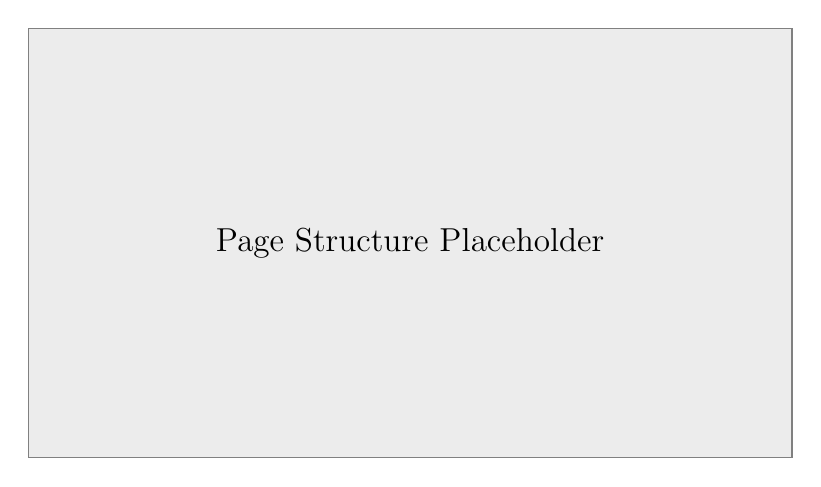
\begin{tikzpicture}
      \node[draw=gray, line width=0.4pt, fill=gray!15,
            minimum width=0.8\textwidth, minimum height=0.45\textwidth,
            inner sep=0pt] (box) {};
      \node at (box) {\large Page Structure Placeholder};
    \end{tikzpicture}
    \caption{Standard Page Structure}
    \label{fig:page-structure}
\end{figure}

This modular structure allows for consistent yet flexible page layouts across the portal.

\subsection{Documentation at the Page Level}
\label{sec:page-documentation}

Pages should document specific workflows and processes. For example, the "Quote Generator" page might include detailed process documentation:

\begin{lstlisting}[language=JSON,caption={Page with Process Documentation},label={lst:process-page-docs}]
{
  "_id": "quote_generation_page",
  "type": "Page",
  "name": {
    "en": "Generate New Quote"
  },
  "description": {
    "en": "This page implements process PROC-SALES-002 for generating new customer quotes. The process requires completion of the customer information form and selection of products from the official catalog. All generated quotes must be approved by a sales manager before being sent to the customer. This process is audited quarterly under audit procedure AUD-Q-004."
  },
  "keywords": {
    "en": "quote, sales process, PROC-SALES-002, audit, compliance"
  }
}
\end{lstlisting}

\subsection{Integrated Ticketing and Feedback}
\label{sec:ticketing}

A professional portal must include a \textbf{ticketing system} that captures and tracks requests beyond products or services. Tickets should also address the \emph{portal structure and behavior} itself (navigation, layout, performance, accessibility, localization), as well as data quality, access/permissions, and feature requests.

Recommended capabilities:
\begin{itemize}
  \item \textbf{Entry points}: a global action in the header (Help/Support), and an \emph{in-context} action near the main content (e.g., “Report an issue with this page”).
  \item \textbf{Automatic context}: include URL, Area/Page/Content identifiers, user locale, device, and current filters/scope when applicable.
  \item \textbf{Classification}: category (product/service, portal structure, portal behavior/UX, data issue, access/permissions, feature request), severity/impact, attachments, and tags.
  \item \textbf{Workflow}: triage, assignment, SLA targets, status, and audit trail. Integrate with quality management and release notes.
  \item \textbf{Discoverability}: use localized \texttt{keywords} and \texttt{description} to improve internal SEO for ticket templates and knowledge-base links.
\end{itemize}

Example of a ticket payload embedding structural context:
\begin{lstlisting}[language=JSON,caption={Ticket with Structural Context},label={lst:ticket-structure}]
{
  "_id": "tick-2025-09-09-1234",
  "type": "Ticket",
  "category": "portal_structure",
  "summary": { "en": "Sidebar filters hidden at 1280px" },
  "description": { "en": "On Customers page, the left filter panel collapses unexpectedly at 1280px width." },
  "scope": {
    "site": "stw_site",
    "area": "sales",
    "page": "customers_list",
    "content": "customers_table"
  },
  "context": {
    "url": "/sales/customers",
    "locale": "en",
    "viewport": "1280x720",
    "filters": { "status": "active" }
  },
  "severity": "medium",
  "status": "new",
  "attachments": [],
  "keywords": { "en": "ux, layout, sidebar, filters" }
}
\end{lstlisting}

This approach ensures issues are actionable and traceable, while keeping the feedback loop close to where users work.

\section{Step 3: Build Pages with Content Blocks}
\label{sec:build-with-content}

The final step is to populate the pages with \textbf{Content (\texttt{STWContent})} blocks. These are the building blocks that display information and provide functionality. A single page will typically be composed of multiple content blocks.

Let's design the public-facing \textbf{"Products"} page from the "Products \& Services" Area. This page needs to be informative and engaging for potential customers. It could be built with the following \texttt{STWContent} blocks:

\begin{enumerate}
    \item \textbf{A Hero Banner}: An eye-catching banner image with a marketing headline. This is a static content block.
    \item \textbf{Product Categories Menu}: A navigation menu, perhaps implemented as tabs or an accordion, that allows users to filter products by category. This content block would use \wbpl{} to dynamically query the list of product categories from a database.
    \item \textbf{Product Listing Grid}: A grid that displays the products. Each item in the grid would show a product image, name, and a short description. This is a highly dynamic content block, driven by a \wbpl{} query that fetches the product data based on the selected category.
    \item \textbf{Featured Products Carousel}: A rotating carousel showcasing new or featured products. This could be driven by a separate, specialized query.
    \item \textbf{Call to Action}: A block encouraging users to "Request a Quote" or "Contact Sales," linking to another page in the portal.
\end{enumerate}

By combining these static and dynamic content blocks, you can create a rich, interactive, and data-driven page that effectively serves the needs of its audience.

\subsection{Documentation at the Content Level}
\label{sec:content-documentation}

Individual content blocks can contain specific field-level instructions and validation rules. For example, a customer information form might include:

\begin{lstlisting}[language=JSON,caption={Content with Field-Level Documentation},label={lst:form-content-docs}]
{
  "_id": "customer_info_form",
  "type": "Content",
  "subtype": "Form",
  "name": {
    "en": "Customer Information"
  },
  "description": {
    "en": "Customer Data Collection Form - FORM-CRM-001. This form collects essential customer information required for quote generation. All fields marked with (*) are mandatory as per our Customer Data Policy CDP-001. Data Validation Rules: Company Name (min 2, max 100 chars), Email (valid business format). Data Protection Notice: Customer data is processed according to GDPR Article 6(1)(b). Data retention period: 7 years."
  },
  "keywords": {
    "en": "customer data, GDPR, validation rules, data quality, mandatory fields"
  }
}
\end{lstlisting}

This multi-level documentation approach ensures that quality management principles, compliance requirements, and operational procedures are seamlessly integrated throughout the portal structure, creating a comprehensive knowledge management system that supports both daily operations and audit requirements.

\subsection{Search Modes and SEO}
\label{sec:search-and-seo}

The localized \texttt{keywords} and \texttt{description} fields on every \wbdl{} element are not just documentation—they power internal SEO within the portal. They improve discoverability in menus and sitemap views, drive search ranking and snippets in \studio{}, and help generate meaningful breadcrumbs and suggestions.

There are two complementary search experiences:
\begin{description}
  \item[Site-wide Search] traverses Areas, Pages, and Content using localized metadata (\texttt{name}, \texttt{keywords}, \texttt{description}) and usage signals. It is typically exposed in the page header and returns cross-area results.
  \item[In-context Search] operates within the active page. It narrows scope to the main body: filtering rows in tables/lists, quick find in forms, text search in rich content, and local help/glossary. Place it near the primary content (e.g., table toolbar or section header) for immediate focus.
\end{description}

Design guidance: keep global search persistent in the header; keep in-context search adjacent to the content it filters. Ensure accessibility (labels, ARIA, keyboard shortcuts like / to focus, Esc to clear) and support localization for both search modes.

\section{Looking Forward}
\label{sec:portal-structure-forward}

This chapter has provided a practical methodology for structuring a web portal by mapping business functions to Areas, user journeys to Pages, and informational needs to Content blocks. This "documentation through structure" approach ensures that the resulting portal is both logical and self-describing.

However, building a successful portal requires more than just technical structure; it requires a specific mindset and an understanding of recurring patterns. The next chapter delves into the learning journey of a portal developer, exploring the key patterns and nomenclature that emerge from experience.
